\chapter{Detalle complementario das probas}
\label{app:probas-complementarias}

Este apéndice amplía a información presentada no Capítulo~\ref{chap:probas} e recolle exemplos representativos das probas realizadas sobre a \gls{api} e a aplicación móbil. Inclúense a organización das probas, algúns dos casos empregados para verificar os compoñentes principais, os comandos empregados e as evidencias obtidas durante as comprobacións automatizadas e manuais.

Os fragmentos de código proceden das probas implementadas no proxecto. Co obxectivo de facilitar a súa lectura, nalgúns casos omítense partes de preparación que non resultan relevantes para comprender o comportamento que se está verificando.

\section{Organización e alcance}

As probas desenvolvéronse sobre diferentes niveis da solución. Na \gls{api} comprobáronse tanto funcións concretas da lóxica de procesamento como o comportamento dos endpoints e das dependencias externas. No cliente avaliáronse os modelos, os modelos de vista, os servizos, a persistencia, o cifrado, os widgets e distintos fluxos nos que interveñen varias capas da aplicación.


\section{Probas da API}

\subsection{Preparación das probas dos endpoints}

Para comprobar os endpoints empregouse TestClient, que permite realizar peticións \gls{http} directamente sobre a aplicación FastAPI durante a execución das probas. As dependencias que requiren comunicación con servizos externos substituíronse por obxectos simulados cando era necesario, permitindo preparar respostas coñecidas e reproducir situacións de éxito e de erro sen depender dunha conexión externa.

No caso de Azure Document Intelligence, o cliente utilizado pola aplicación substitúese por un MagicMock. Desta maneira pódense construír respostas coa mesma estrutura que as devoltas polo servizo e comprobar posteriormente como son procesadas pola \gls{api}.

\begin{lstlisting}[
    language=Python,
    caption={Preparación do cliente de FastAPI e simulación do cliente de Azure},
    label={lst:mock-azure}
]
def setUp(self):
    self.azure = MagicMock()
    app.state.doc_intel_client = self.azure
    self.client = TestClient(app)

def responder_con(self, fields):
    documento = SimpleNamespace(fields=fields)
    resultado = SimpleNamespace(documents=[documento])
    self.azure.begin_analyze_document \
        .return_value.result.return_value = resultado

def enviar(self, tipo="image/jpeg"):
    return self.client.post(
        "/extraccion/",
        files={"file": ("informe", b"bytes", tipo)},
    )
\end{lstlisting}

Esta preparación permite reproducir, entre outros casos, unha extracción correcta, resultados incompletos, valores cunha confianza insuficiente ou erros producidos durante a comunicación co servizo.


\subsection{Procesamento e validación dos datos}

As probas da lóxica interna verifican o tratamento dos datos extraídos antes de construír a resposta enviada ao cliente. Comprobáronse especialmente a interpretación das doses, o tratamento das datas e os cambios de ano, a detección dos días de control e as validacións realizadas sobre campos como o \gls{inr}.

Tamén se incluíron entradas incorrectas ou incompletas co obxectivo de comprobar que a aplicación non produce resultados incoherentes cando a información recibida non é válida.

Como exemplo, o seguinte caso comproba a corrección da data correspondente a un control cando a data detectada non coincide coa próxima visita indicada na folla.

\begin{lstlisting}[
    language=Python,
    caption={Comprobación da data correspondente a un control},
    label={lst:api-control-data}
]
for data_control, data_esperada in (
    ("10 ENE CONTROL", "2026-01-10"),
    ("09 ENE CONTROL", "2026-01-10"),
):
    with self.subTest(data_control=data_control):
        self.responder_con({
            "fecha visita": campo("01/01/2026"),
            "prox visit": campo("10/01/2026"),
            "DOSE": campo(value_array=[
                fila(LUNES=campo(data_control))
            ]),
        })

        resposta = self.enviar()

        self.assertEqual(resposta.status_code, 200)
        self.assertEqual(
            resposta.json()["calendario"][0]["data"],
            data_esperada,
        )
\end{lstlisting}


\subsection{Preprocesamento das imaxes}

O módulo de preprocesamento probouse de maneira independente antes da chamada ao servizo de extracción. Para iso empregáronse imaxes creadas especificamente para as probas e sometidas a diferentes transformacións.

Comprobouse o comportamento con documentos rectos, inclinados e con deformación de perspectiva, así como con ficheiros ou dimensións que non permitían aplicar correctamente o procesamento. Tamén se verificou que un erro nesta etapa non impida continuar coa extracción, conservando neste caso o ficheiro orixinal.

Estas probas resultan especialmente relevantes porque o preprocesamento inclúe diferentes ramas en función das características da imaxe recibida.


\subsection{Notificacións e dependencias externas}

As chamadas ao \gls{sdk} de Firebase simuláronse durante as probas automatizadas. Isto permite comprobar a información empregada para construír a notificación, o token de destino e o tratamento dos posibles erros sen enviar mensaxes reais.

\begin{lstlisting}[
    language=Python,
    caption={Simulación do envío dunha notificación mediante Firebase},
    label={lst:mock-firebase}
]
@patch("app.routers.notificar.messaging.send",
       return_value="mensaxe-456")
@patch("app.routers.notificar.messaging.Message")
def test_aviso_desconecido_sen_notificacion(
        self, message_mock, _send_mock):

    resposta = self.client.post(
        "/notificar/enviar",
        json={**self.datos, "tipo_aviso": "OUTRO"},
    )

    self.assertEqual(resposta.status_code, 200)
    self.assertIsNone(
        message_mock.call_args.kwargs["notification"]
    )
\end{lstlisting}

Ademais dos casos correctos, provocáronse erros durante o envío para comprobar que a \gls{api} devolve a resposta correspondente.

O arranque da aplicación tamén foi probado baixo diferentes configuracións de Azure, Firebase e Key Vault, comprobando tanto a carga das credenciais desde as variables de contorna como a recuperación dos segredos externos.


\section{Probas do cliente Flutter}

\subsection{Comunicación coa API}

A comunicación \gls{http} probouse substituíndo o cliente real por un MockClient. Deste modo é posible interceptar as peticións xeradas pola aplicación e comprobar o método \gls{http} empregado, a ruta, as cabeceiras e os datos enviados.

\begin{lstlisting}[
    caption={Comprobación dunha petición realizada polo cliente},
    label={lst:flutter-mock-http}
]
final api = ApiService(
  client: MockClient((request) async {
    expect(request.method, 'POST');
    expect(request.url.path,
        AppConstants.endpointEnviarNotif);

    expect(jsonDecode(request.body), {
      'token_destino': 'token',
      'payload': 'cifrado',
      'tipo_aviso': 'TOMA_CONFIRMADA',
    });

    return http.Response('', 200);
  }),
);
\end{lstlisting}

Tamén se simularon respostas incorrectas do servidor e erros de conexión para comprobar que estes casos son tratados pola aplicación.


\subsection{Persistencia dos datos}

As probas de persistencia executan unha base SQLite destinada exclusivamente á suite de probas. Antes de cada caso elimínanse os datos anteriores, garantindo que os resultados non dependan da execución doutros tests.

Entre os escenarios comprobados encóntranse o gardado e recuperación dunha análise, o rexistro dunha toma, a conservación dos estados cando se importa novamente a mesma folla e a substitución da pauta cando se incorpora unha folla diferente.

O seguinte exemplo comproba que unha toma rexistrada fóra da hora prevista se conserva despois de importar novamente a mesma pauta.

\begin{lstlisting}[
    caption={Conservación dunha toma ao reimportar a mesma pauta},
    label={lst:flutter-reimportacion}
]
final analise = crearAnaliseProba();

await servizo.gardarAnalise(analise);

await servizo.rexistrarToma(
  data: '2026-08-21',
  instante: DateTime(2026, 8, 21, 20, 10),
  desviacionMinutos: 10,
  foraDeHora: true,
);

await servizo.gardarAnalise(analise);

final rexistros =
    await servizo.obterRexistrosCumprimento();

expect(
  rexistros.single['estado'],
  'TOMADA_FORA_HORA',
);
\end{lstlisting}


\subsection{Cifrado e integridade das mensaxes}

As operacións criptográficas empregadas durante as probas son operacións \gls{aesgcm} reais. Só se substitúe o almacenamento empregado para conservar as claves, permitindo executar a suite sen depender do almacenamento seguro do dispositivo.

Comprobouse que os datos poden descifrarse coa clave correspondente e que unha mensaxe modificada, un tipo de aviso diferente ou unha clave incorrecta provoca o rexeitamento da mensaxe.

\begin{lstlisting}[
    caption={Comprobación do cifrado e descifrado mediante AES-GCM},
    label={lst:flutter-cifrado}
]
const payload = '{"dose":"1/2","inr":"2.4"}';

final envelope = await servizo.cifrarPayload(
  vinculacion: vinculacion,
  tipoAviso: 'ESTADO_COMPLETO',
  payload: payload,
);

expect(envelope, isNot(contains('2.4')));

final resultado =
    await servizo.descifrarPayloadConClave(
  envelope: envelope,
  tipoAviso: 'ESTADO_COMPLETO',
  claveBase64: clave,
);

expect(resultado.contido, payload);
\end{lstlisting}


\subsection{Planificación dos recordatorios}

A lóxica encargada de decidir que recordatorios deben programarse probouse independentemente do complemento nativo de Android. As datas e horas utilizadas nos casos de proba son fixas, o que permite obter sempre o mesmo resultado independentemente do momento no que se execute a suite.

Comprobáronse diferentes estados das tomas e verificouse que unha toma xa confirmada non xere novos avisos.

\begin{lstlisting}[
    caption={Comprobación da planificación dos recordatorios},
    label={lst:flutter-planificador}
]
final avisos = PlanificadorRecordatorios.crear(
  agora: DateTime(2026, 7, 28, 10),
  hora: '20:00',
  datasConToma: const [
    '2026-07-28',
    '2026-07-29',
  ],
  estados: const {
    '2026-07-28': 'TOMADA',
  },
);

expect(
  avisos.every(
    (aviso) => aviso.data == '2026-07-29'
  ),
  isTrue,
);
\end{lstlisting}


\subsection{Probas da interface}

As probas de widgets permitiron comprobar o comportamento das principais pantallas sen necesidade de executar toda a aplicación nun dispositivo. Simuláronse interaccións da persoa usuaria, como pulsacións, introdución de datos ou navegación entre pantallas, verificando posteriormente o estado mostrado.

Entre os elementos comprobados atópanse os formularios de configuración, a pantalla de revisión dos datos extraídos, o calendario, o progreso do tratamento, os estados de carga e as diferentes mensaxes de erro.


\section{Execución das probas automatizadas}

Ademais de comprobar casos individuais, executáronse as suites completas para verificar que o conxunto das probas finalizaba correctamente e obter a cobertura acadada.


\subsection{Execución da API}

As probas da \gls{api} executáronse desde a raíz do repositorio empregando Coverage.py:

\begin{lstlisting}[
    caption={Execución das probas e cálculo da cobertura da API}
]
$env:PYTHONPATH="$PWD;$PWD\server"

python -m coverage run \
    --source=server/app \
    -m unittest discover \
    -s server/test \
    -p test_*.py

python -m coverage report -m
\end{lstlisting}

A execución completouse correctamente e o informe mostrou unha cobertura global do 96,1 \%. Todos os módulos alcanzaron unha cobertura completa agás o módulo de preprocesamento, no que quedaron algunhas ramas sen executar.

\begin{figure}[htbp]
    \centering
    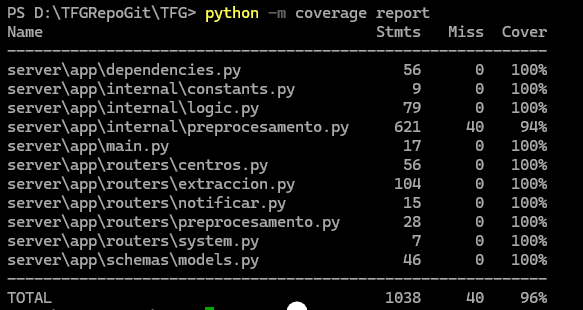
\includegraphics[
        width=0.92\textwidth
    ]{imaxes/09-Probas/execucion-api.png}
    \caption{Resultado da execución das probas e da cobertura da API}
    \label{fig:execucion-probas-api}
\end{figure}

Na Figura~\ref{fig:execucion-probas-api} pode observarse tanto a finalización correcta da suite como a cobertura obtida nos diferentes módulos.


\subsection{Execución do cliente Flutter}

No cliente empregouse o comando de probas de Flutter coa xeración simultánea do ficheiro LCOV:

\begin{lstlisting}[
    caption={Execución das probas automatizadas de Flutter}
]
flutter test --no-pub --coverage
\end{lstlisting}

A suite executou correctamente 114 probas. O ficheiro LCOV xerado contabilizou 2447 liñas instrumentadas, das cales 1781 foron executadas, o que representa unha cobertura global do 72,8 \%.

\begin{figure}[htbp]
    \centering
    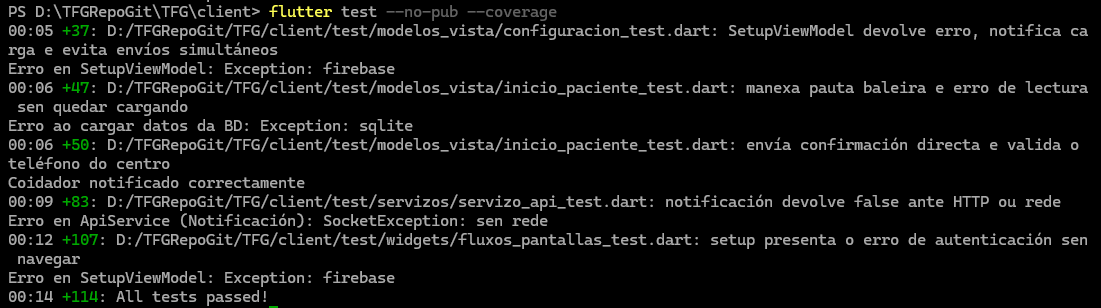
\includegraphics[
        width=1\textwidth
    ]{imaxes/09-Probas/execucion-flutter.png}
    \caption{Resultado da execución das probas automatizadas de Flutter. As mensaxes de erro corresponden a casos probados de forma intencionada. En total, superáronse correctamente as 114 probas.}
    \label{fig:execucion-probas-flutter}
\end{figure}

\section{Comprobacións en dispositivos Android}

As probas automatizadas non permiten reproducir completamente determinadas funcionalidades que dependen do sistema operativo ou da interacción entre dispositivos. Por este motivo realizáronse tamén probas manuais sobre os principais fluxos da aplicación.

As comprobacións incluíron:

\begin{itemize}
    \item completar a configuración inicial como paciente e como supervisor;
    \item incorporar unha folla mediante a cámara, a galería e un documento \gls{pdf};
    \item revisar e modificar os datos obtidos antes de gardar a pauta;
    \item comprobar a persistencia da información despois de pechar e volver abrir a aplicación;
    \item consultar o calendario e confirmar unha toma;
    \item comprobar a programación e recepción dos recordatorios;
    \item vincular paciente e supervisor mediante un código \gls{qr};
    \item sincronizar a pauta e os estados das tomas entre dous dispositivos;
    \item comprobar a recepción das notificacións entre ambos;
    \item eliminar unha vinculación e verificar a actualización dos dous dispositivos;
    \item provocar erros de comunicación ou empregar documentos non válidos para comprobar as mensaxes mostradas.
\end{itemize}

Estas probas complementan a cobertura automatizada, especialmente nas funcionalidades que precisan acceso á cámara, ás notificacións do sistema e á comunicación mediante Firebase.


\subsection{Evidencias das probas manuais}

A Figura~\ref{fig:proba-vinculacion} mostra unha das comprobacións realizadas durante o proceso de vinculación entre paciente e supervisor mediante código \gls{qr}.

 \begin{figure}[htbp]
     \centering
     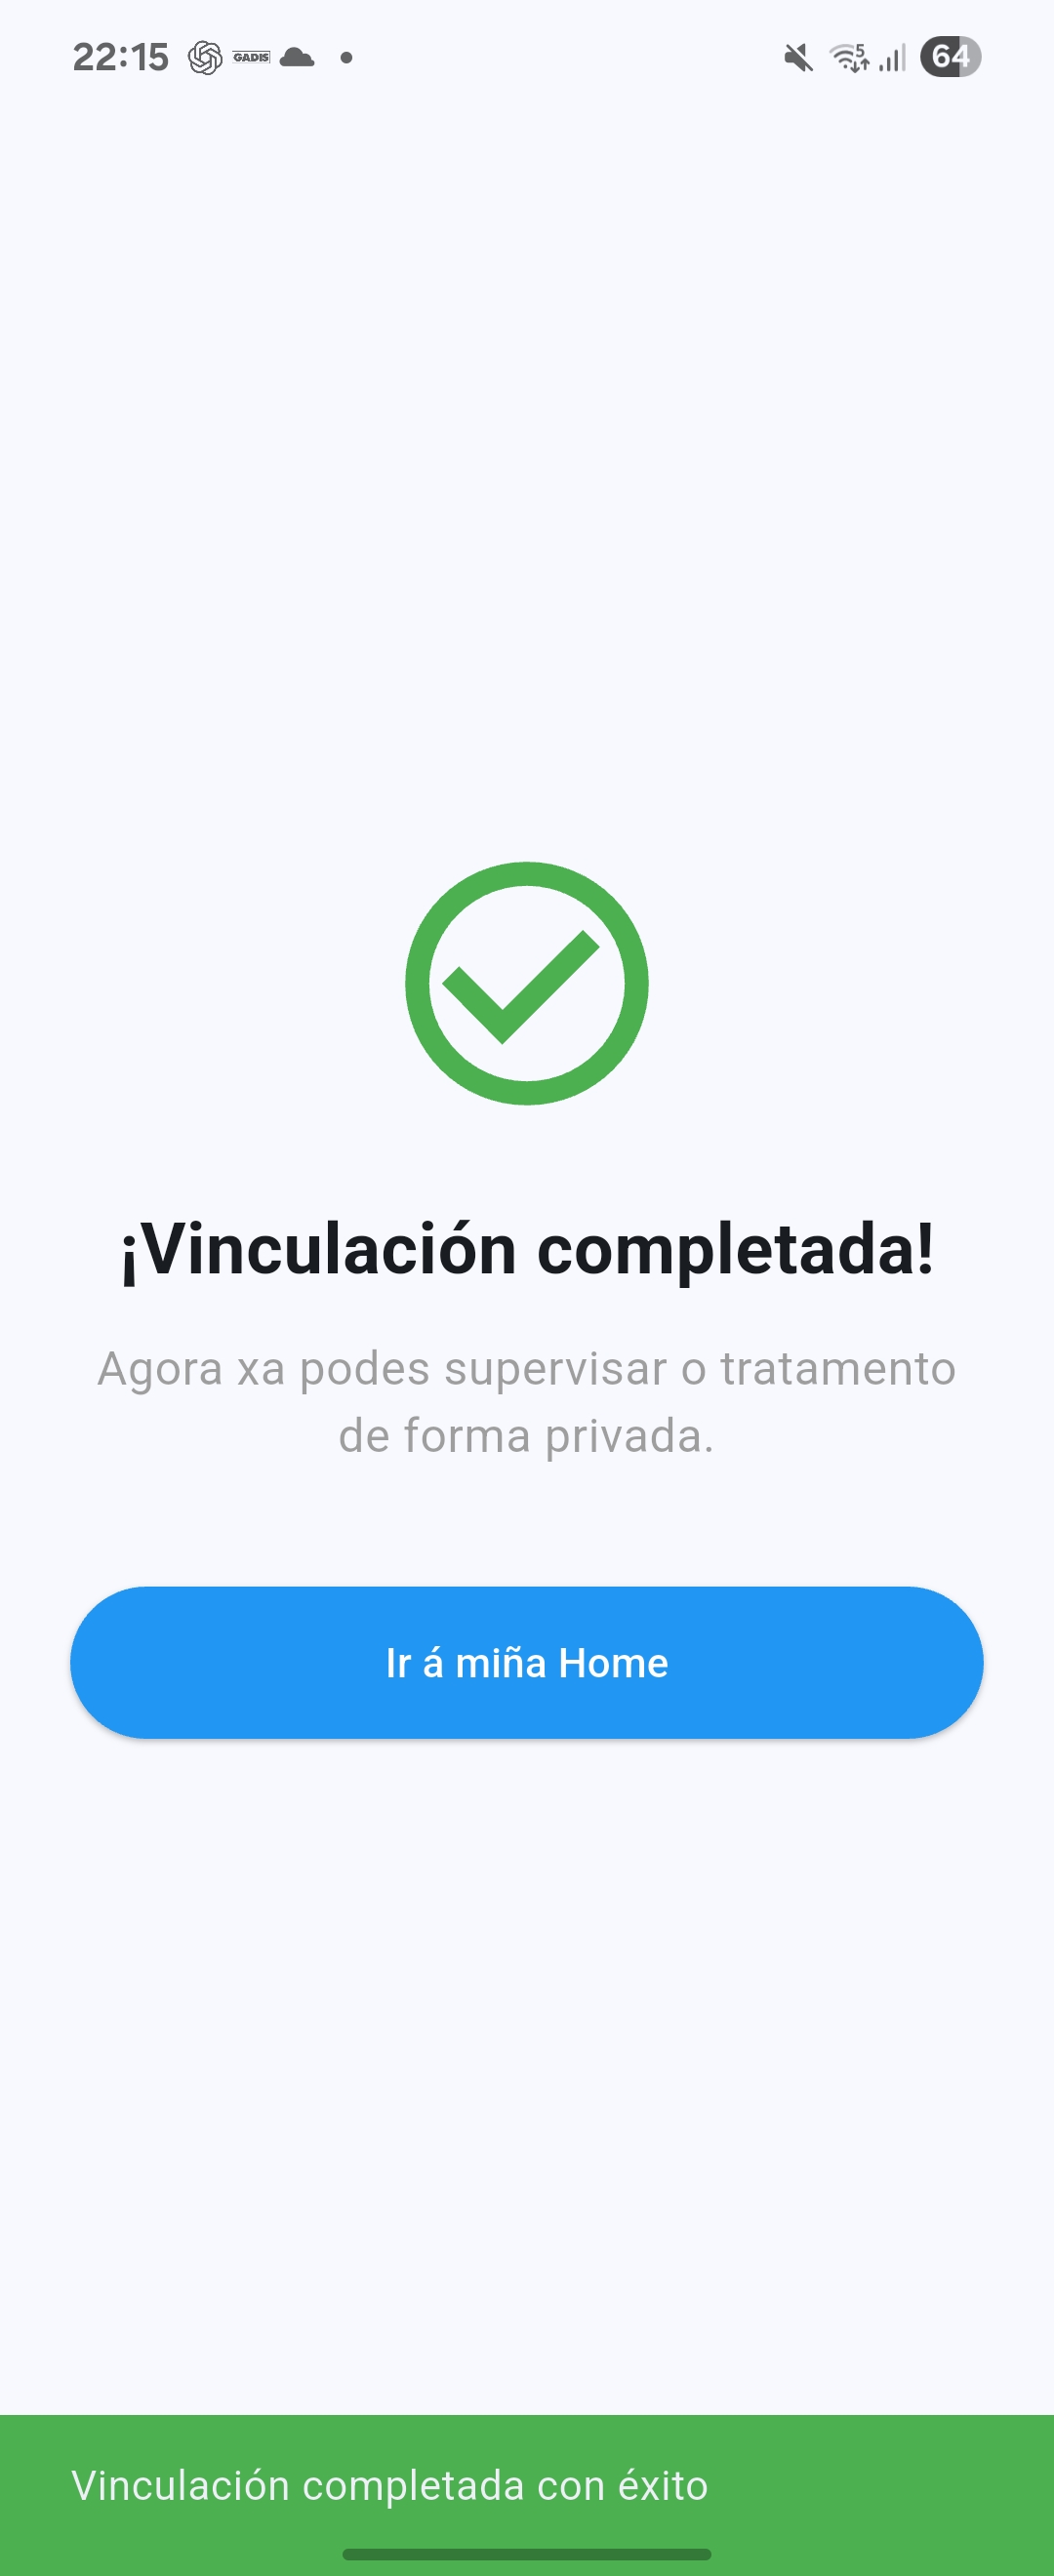
\includegraphics[width=0.5\textwidth]{imaxes/09-Probas/anexo/vinculación-correcta.jpg}
     \caption{Proba da vinculación entre paciente e supervisor}
    \label{fig:proba-vinculacion}
 \end{figure}


Tamén se comprobou a recepción real dos avisos xerados pola aplicación no sistema de notificacións de Android.


\begin{figure}[htbp]
    \centering

    
\includegraphics[width=0.55\textwidth]{imaxes/09-Probas/anexo/toma-confirmada.jpg}

    \vspace{0.4cm}

    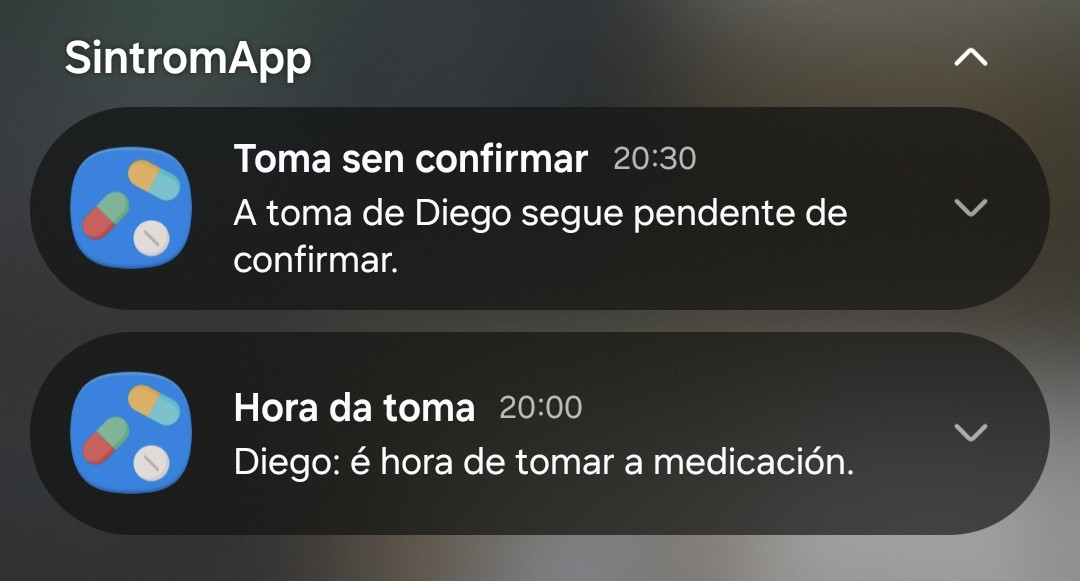
\includegraphics[width=0.55\textwidth]{imaxes/09-Probas/anexo/tomas-sen-confirmar.png}

    \caption{Confirmación dunha toma e recepción dunha notificación durante as probas en dispositivo Android.}
    \label{fig:proba-notificacion}
\end{figure}


Finalmente, a sincronización entre os dous roles comprobouse realizando a toma dunha dose no dispositivo do paciente e verificando posteriormente a actualización da información no dispositivo da persoa supervisora. 

\begin{figure}[htbp]
    \centering

    \begin{subfigure}[b]{0.48\textwidth}
        \centering
        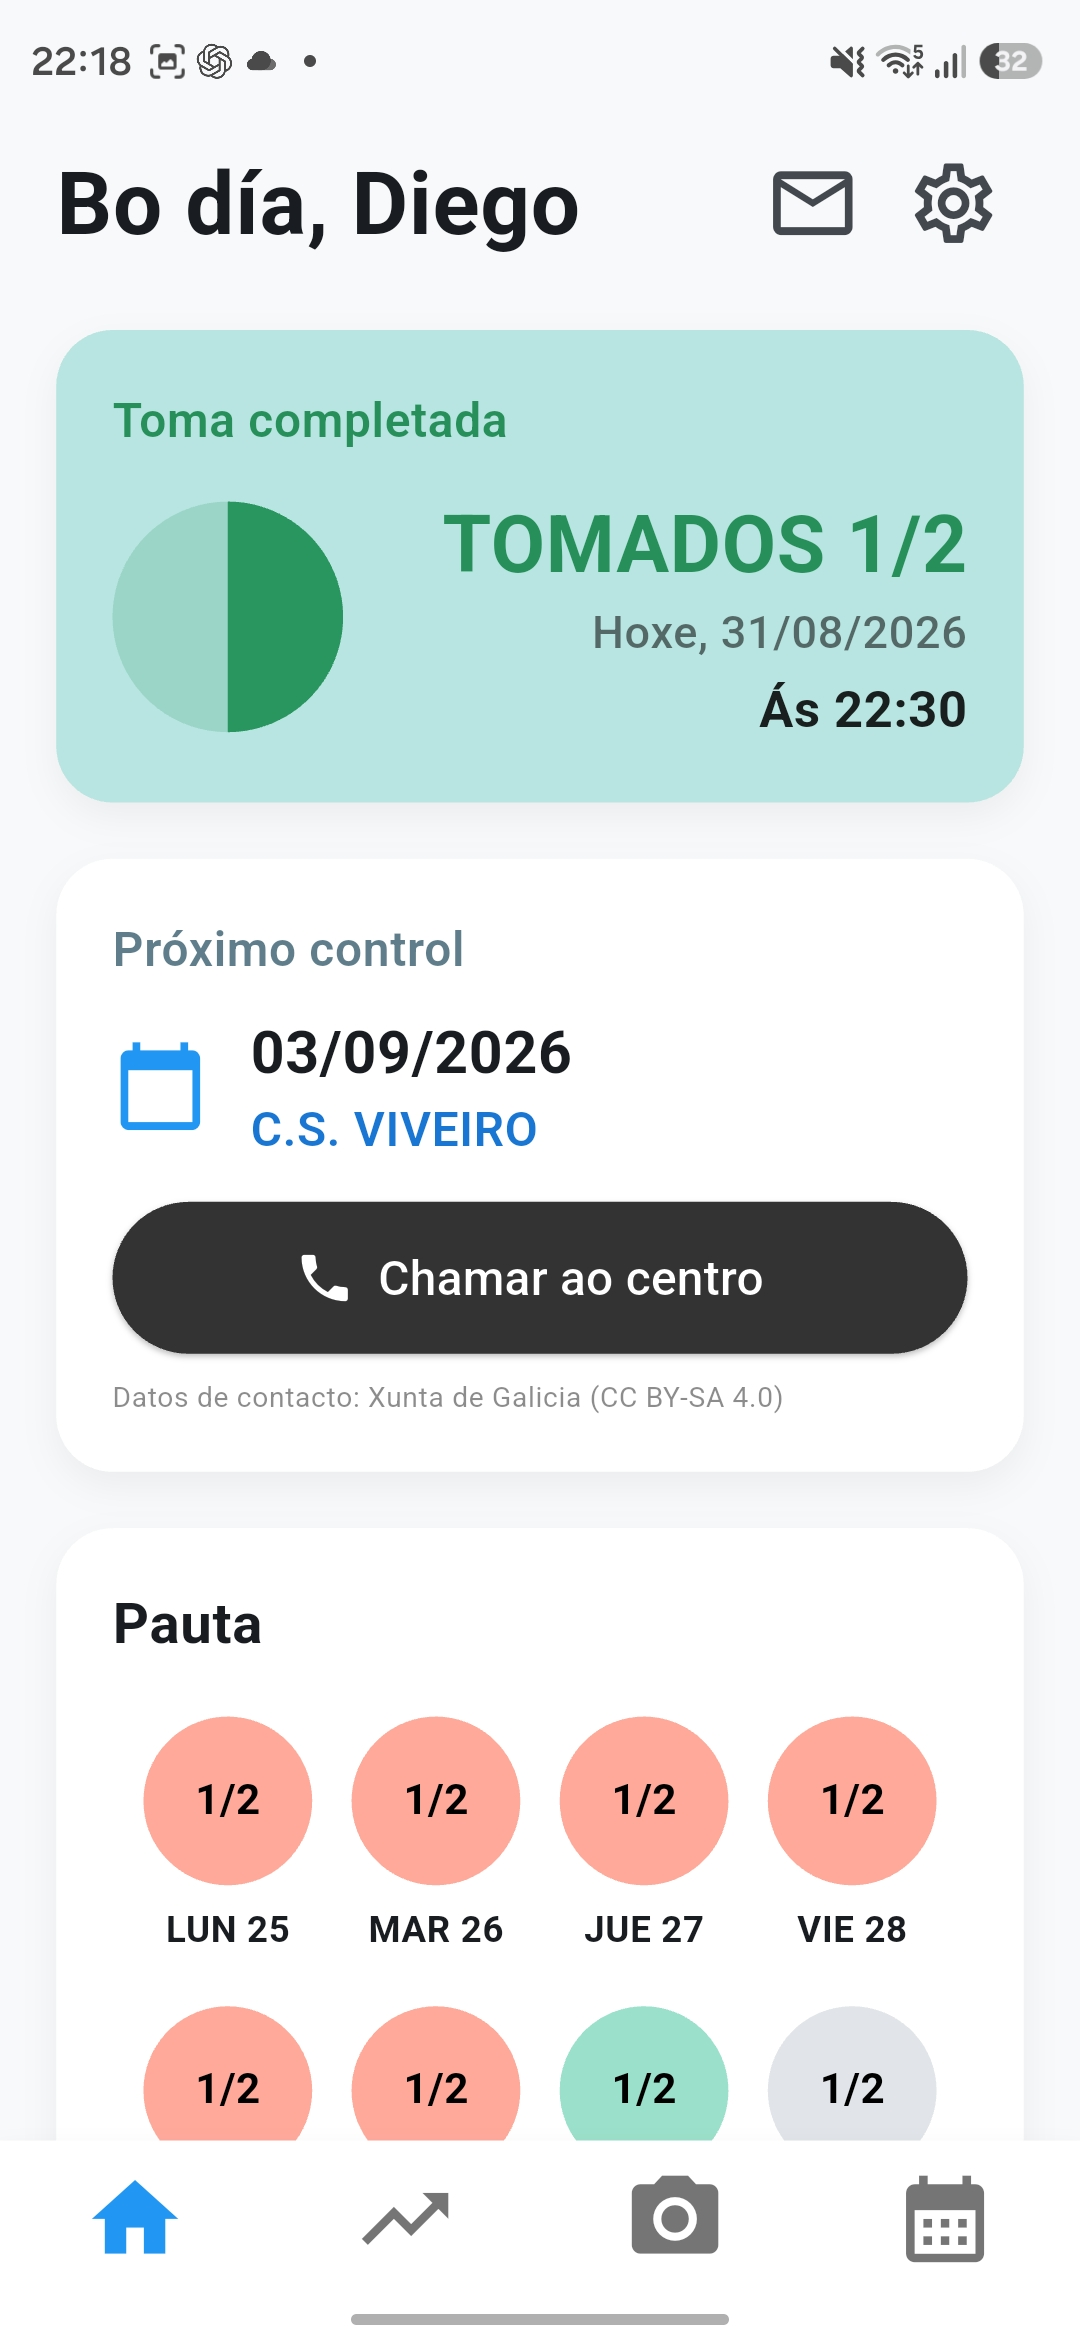
\includegraphics[width=\textwidth]{imaxes/09-Probas/anexo/toma-confirm.jpg}
        \caption{Vista do paciente.}
        \label{fig:proba-sincronizacion-paciente}
    \end{subfigure}
    \hfill
    \begin{subfigure}[b]{0.48\textwidth}
        \centering
        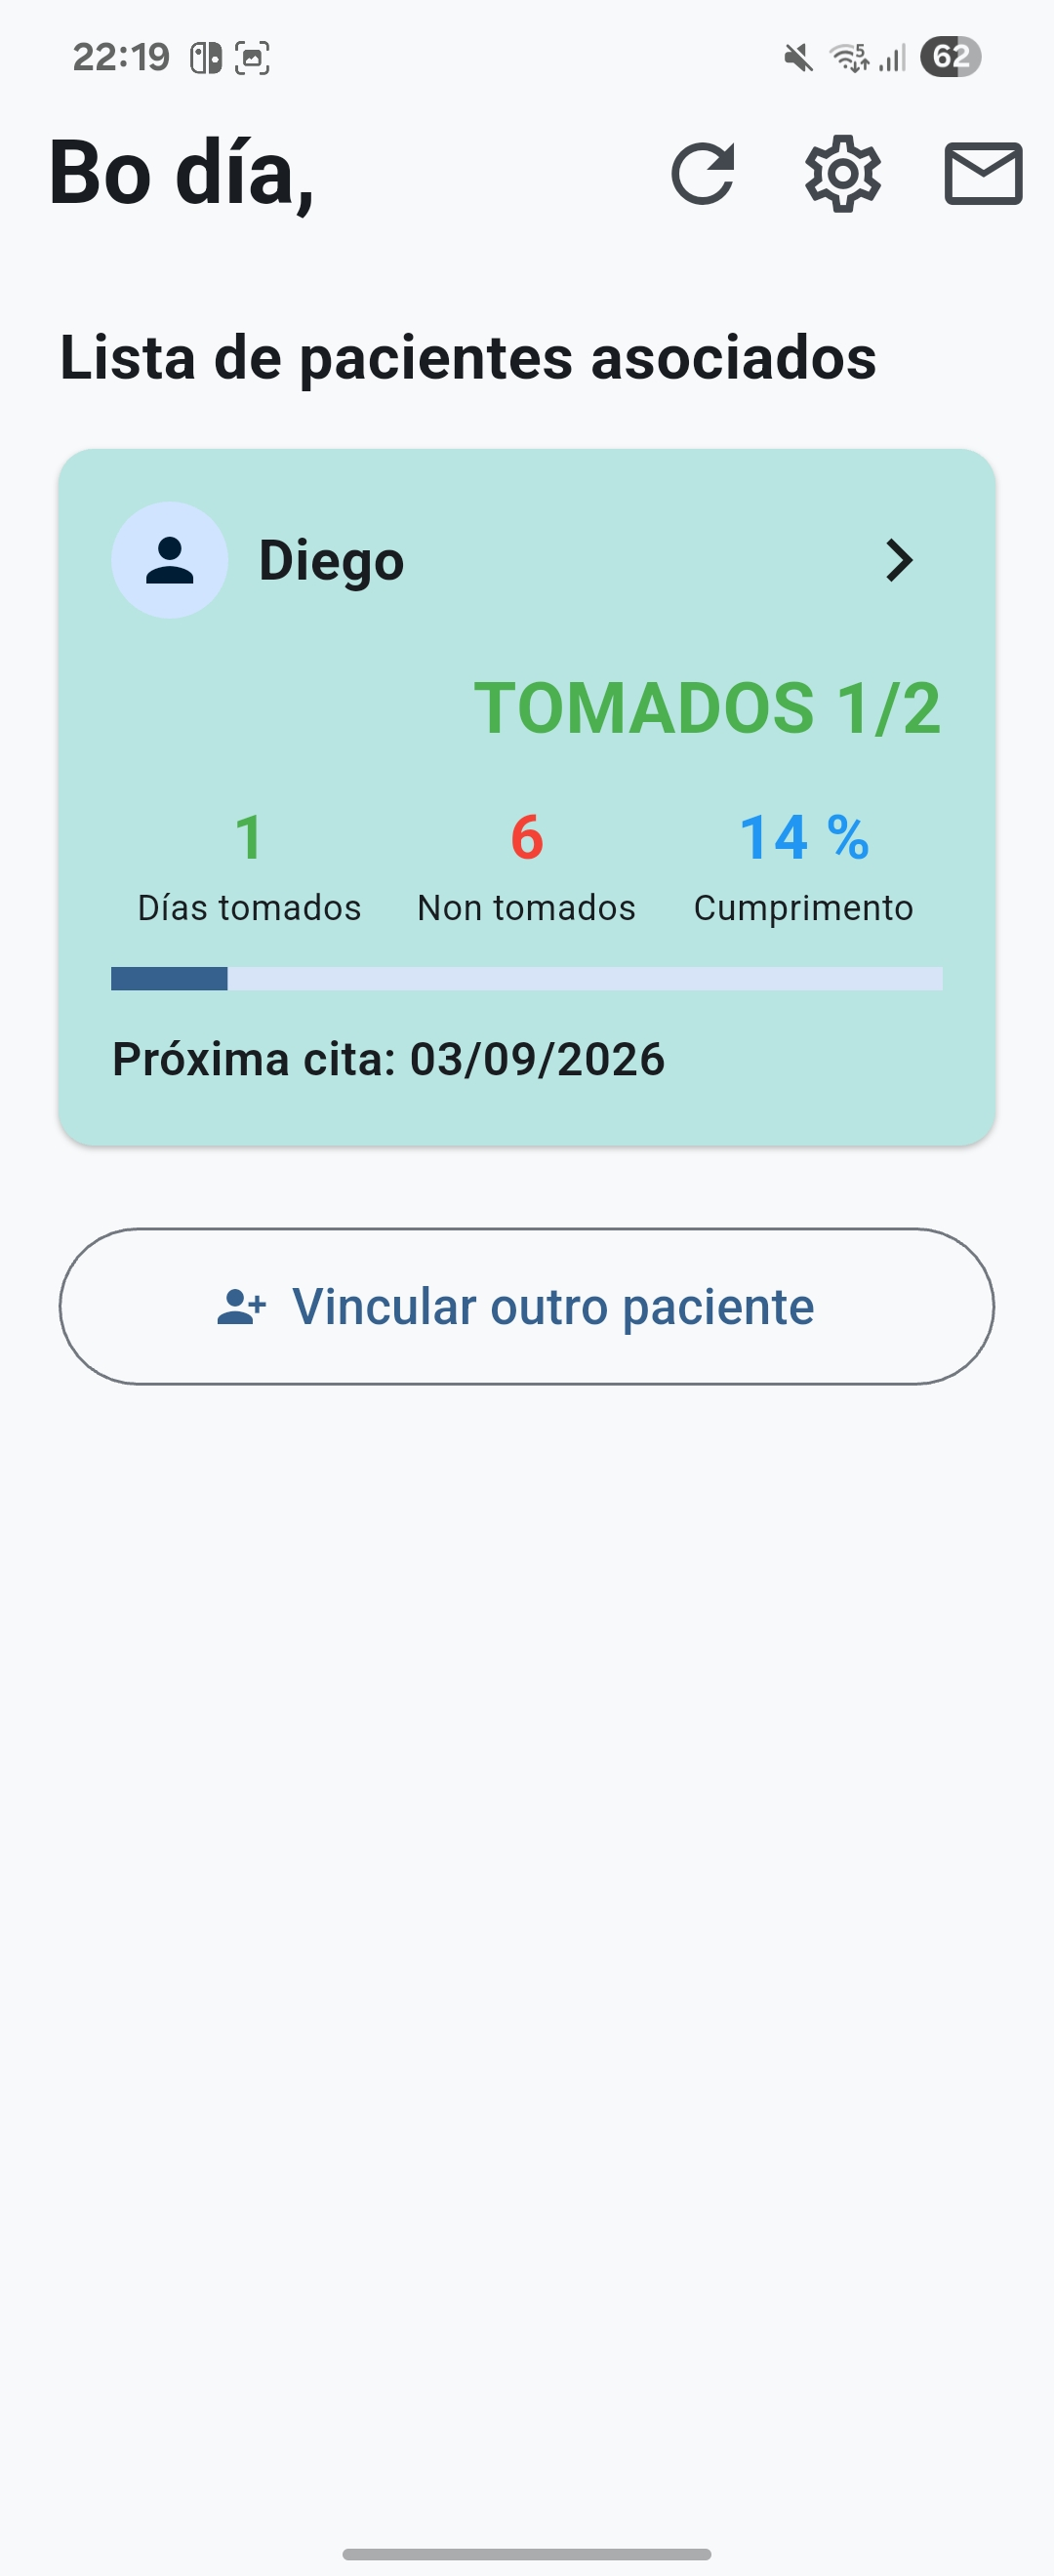
\includegraphics[width=\textwidth]{imaxes/09-Probas/anexo/toma-confirm-sup.jpg}
        \caption{Vista do supervisor.}
        \label{fig:proba-sincronizacion-supervisor}
    \end{subfigure}

    \caption{Comprobación da sincronización entre paciente e supervisor.}
    \label{fig:proba-sincronizacion}
\end{figure}



En conxunto, estas evidencias permiten complementar os resultados das probas automatizadas e verificar os fluxos que dependen directamente das funcionalidades proporcionadas polos dispositivos Android.

